Lantiv Timetabling Turbo 7 er et skemaplanlægningsprogram, der med hensyn til nogle begrænsninger angivet af brugeren, kan udvikle et skema til blandt andet folkeskoler. For hver begrænsning kan brugeren angive en minimum, maksimum og ønsket værdi. En variation af den ønskede værdi bliver af programmet registreret som en mindre overtrædelse mens en værdi, der ligger under minimumsværdien eller over maksimumsværdien, bliver registreret som en alvorlig overtrædelse. Programmet starter med at afsætte kort tid til løsning af overtrædelser, hvorefter den afsatte tid stiger for at løse de sværere overtrædelser. Denne proces stopper, når programmet enten har løst alle overtrædelser, eller den afsatte tid er nået. Hvis overtrædelser af brugerens begrænsninger ikke kan undgås, bliver der lavet et kompromis, hvor programmet hovedsageligt forsøger, at overholde de begrænsninger, brugeren har angivet med høj prioritet, mens overtrædelser af begrænsninger med lav prioritet bliver accepteret. Begrænsningerne kan tilpasses af brugeren, efter skemaet er genereret, og programmet vil levere nogle tilpassede løsninger som forslag. Det oprindelige skema vil kun blive slettet, hvis en af disse løsninger accepteres af brugeren. Under processen kan brugeren bestemme, hvor meget de tilpassede skemaer må variere fra det oprindelige. Der kan f.eks. stilles et krav om, at programmet kun ændrer lektionerne for en enkelt lærer. I dette tilfælde vil ingen af de tilpassede forslag have ændret i andre dele af skemaet. Når skemaet er genereret, er det også muligt for brugeren selv, at tage fat i en lektion og flytte den. Her vil programmet vise, hvor lektionen kan placeres uden at forårsage dobbeltbookninger af lokaler, lærere eller klasser. Hvis brugeren placerer en lektion, der forårsager en konflikt, bliver problemet forklaret i detaljer af programmet. Hvis det er en dobbeltbookning, er der mulighed for at slette en af lektionerne eller accepterer dobbeltbookningen.\footfullcite{lantiv2016}
\begin{figure}[!h]
  \centering
  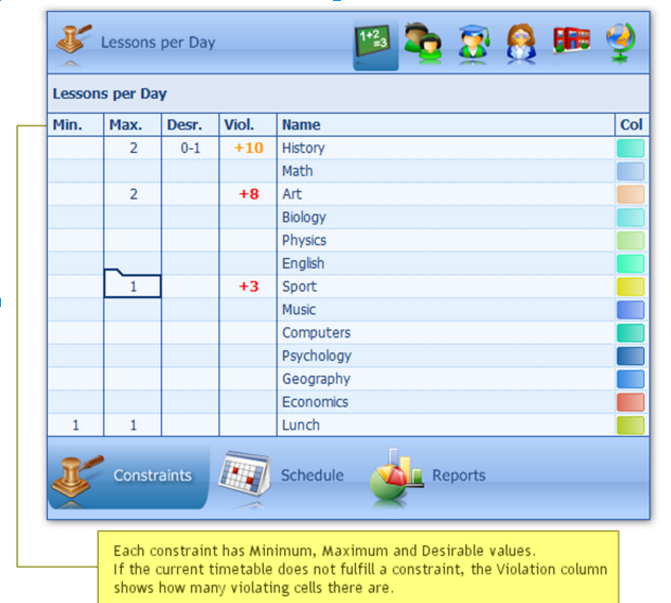
\includegraphics[scale = 0.8]{partials/graphics/LANTIV.png}
    \caption{Eksempel på skemplanlægning i Lantiv.\footfullcite{lantivb}}
  \label{fig:lantiv}
\end{figure}